\documentclass[12pt]{article}
\usepackage[english]{babel}
\usepackage[numbers]{natbib}
\usepackage{graphicx}
\usepackage{xcolor}
\usepackage{sectsty}
\usepackage{float}
\bibliographystyle{apalike}
\setcitestyle{open={[},close={]}}
\sectionfont{\color{DarkBlue}} 
\subsectionfont{\color{LightBlue}}
\subsubsectionfont{\color{LightBlue}}
\paragraphfont{\color{LightBlue}}
\subparagraphfont{\color{LightBlue}}
\definecolor{DarkBlue}{HTML}{4a5a8a}
\definecolor{LightBlue}{HTML}{4f81bf}

\begin{document}
\begin{titlepage}
\begin{flushleft}
\vspace*{1cm}
\Huge
\textbf{Cretaceous Gardens Controller}\\
\vspace{1cm}
\Huge
\textit{Requirements Definition Document}\\
\vspace{1cm}
\Large
\textit{RDD Version 3.0}\\
\vspace{5cm}
\LARGE
Team \#3\\
29 October 2019
\vfill
\Huge
\textbf{CS 460 Software Engineering}
\end{flushleft}
\end{titlepage}
\normalsize
\tableofcontents
\newpage
\section{Introduction}
\paragraph{} The Tyrannosaurus Rex lives among us once again and the opportunity 
to provide an incredible experience has become a reality. The world will be able 
to experience that of which, until now, has only been dreamt. The Cretaceous Gardens
experience will begin the second a visitor steps off the boat and onto the Isla 
Trueno. The visitor will be immersed in Cretaceous Gardens' unique, technological 
advancements: a truly one-of-a-kind luxurious experience. By the time they leave 
they will be already planning their next visit. 

\paragraph{} The purpose of this document is to define the requirements for the 
development of Cretaceous Gardens Controller (CGC) for our billionaire philanthropists 
customers in their new theme park on Isla Trueno near Costa Rica. The CGC is the main 
controller for components like the pay kiosks, cars, and electric fence. The CGC must 
provide sufficient safety, a great user experience, and ought to efficient.

\paragraph{}  Section \ref{obj} outlines the main objectives of the project, 
section \ref{sys} the overall system organization through a high level depiction, 
section \ref{int} outlines interfaces, section \ref{cap} contains the capabilities 
of the system, section \ref{con} provides all known design constraints, and the 
final section provides a reference for potentially unknown terms within the document 
\footnote{Introduction by Anas and Siri.}.  

\section{Objectives}
\label{obj}
\paragraph{} \textit{Four objectives believed to be critical for an 
optimal implementation of a \textit{Cretaceous Gardens Controller} are identified 
here\footnote{Objectives by Anas, Siri and Zeke.}.}
 
	\subsection{Safety}\label{saf}
	\paragraph{} The main objective of the CGC is to provide safe and reliable 
	experiences for the client and its end users. Whether it be electric fences 
	or autonomous vehicles, ensuring safety is of highest priority. The end user
	ought to feel completely safe as should the client whose liability depends on
	this aspect.

	\subsection{Positive User Experience}\label{use}
	\paragraph{} The realization of positive user experiences, in large part, 
	depends on the seamlessness between subsequent interactions with each component
	of a system. For guests, the CGC should be as unimposing as possible in order
	to permit them the fullest immersion offered by Cretaceous Gardens. For the client,
	the system should provide peace of mind that the investment is worthwhile.

	\subsection{Maintainability}\label{mai}
	\paragraph{} The states of the CGC and all \textit{nodes} with which it is to
	communicate should be readily accessible and intelligible. The availability  
	of this information will directly impact the diagnostic and repair speeds 
	anywhere within the system.
	
	\subsection{Efficiency}\label{eff}
	\paragraph{} The CGC is to engender high efficiency and robust functionality. 
	Self-driving cars, pay kiosks, camera system, the global positioning system, 
	electric fence panels, and all other nodes with which the CGC is to interact 
	must not be burdened by inefficiencies of the CGC. On the contrary, the system
	should be expected to gracefully handle nodal malfunctions, failures, or
	inefficiencies.




\section{Overall System Organization} 
\label{sys}
\paragraph{} The CGC will be centralized\footnote{System Organization 
by Anas, Santi, and Siri.} and will manage all relevant components. Figure 
\ref{fig:blackbox} shows a black box diagram of the CGC. The CGC receives inputs 
from sensors, user interfaces, and emergency systems like the \textit{Global 
Alarm System} and responds through appropriate output actions as described 
below.

%%%%%%%%%%%%%%%%%%%%%%%%%%%%%
\paragraph{} The Cretaceous Garden Controller will have 5 self-driving cars, 
transporting people from south to the Exhibit Area (North of the Island). In 
the south of the Island is allocated a Kiosk where the clients can buy their tickets 
giving them access  to the cars and the Exhibition. The Kiosk will record the sales 
and provide to the guest a token device.
%%%%%%%%%%%%%%%%%%%%

\paragraph{} The CGC will control the position the T-Rex via GPS and
cameras. In case of one electric feces fails the emergency plan will be activated,
making sound the alarms and the cars picking people and going to the south,
there will be available 5 more self-driving cars in case of emergency in the 
North.


\begin{figure}[H]
	\centerline{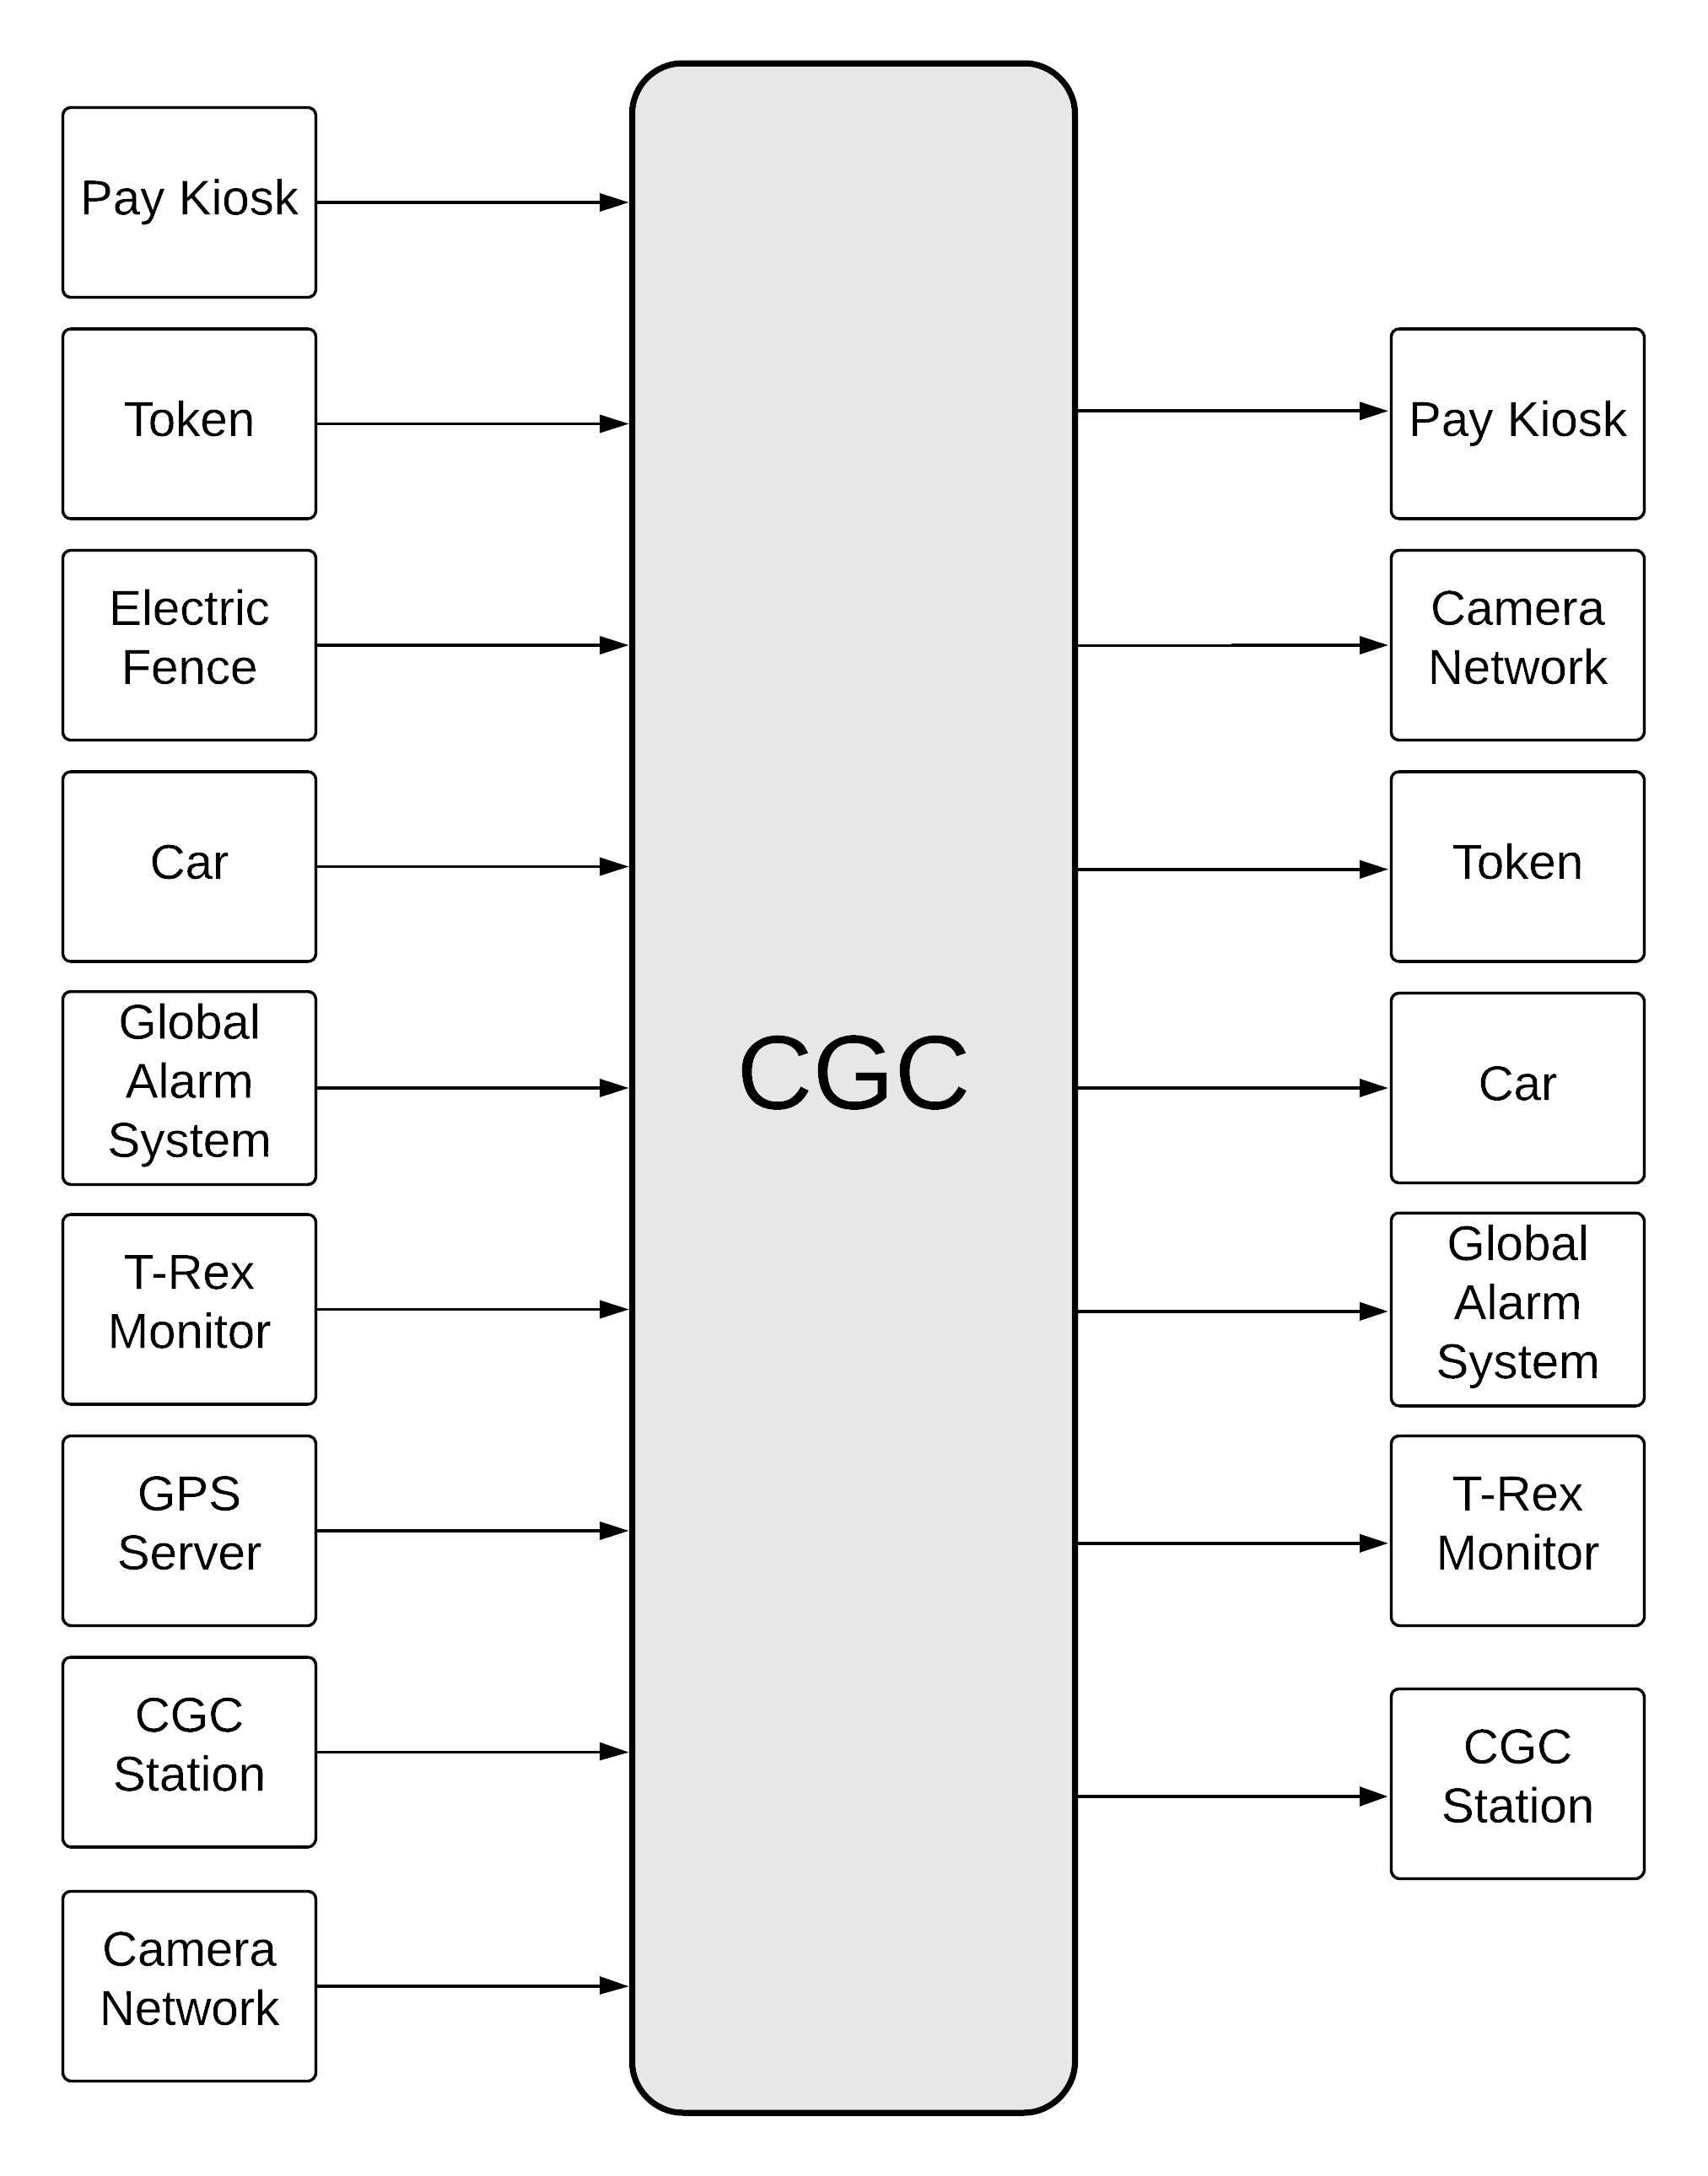
\includegraphics[scale=.17]{CGCBlackBox.png}}
	\caption{A black box of high-level inputs and outputs of the \textit{CGC}.}
	\label{fig:blackbox}
\end{figure}
\vfill
\pagebreak

\section{Interfaces}
\label{int}
\paragraph{} \textit{The interfaces are broken\footnote{Interfaces by Siri 
and Anas.} up into main systems. They may be composed of their own 
sensors but said sensors do not interface with the CGC. The following list of interfaces 
list their sensors, hardware, and features.}

	\subsection{Pay Kiosk}
	\paragraph{} \textit{The purpose of the the Pay Kiosk interface is to connect 
	the physical Pay Kiosks to the CGC,which is composed of sensors and other hardware.}
			
	\paragraph{Sensors}
	\begin{list}{}{}
		\item \textbf{Touch Screen: }used to sense user interaction. 
		\item \textbf{Credit Card: }accepts all major credit/debit cards. 
		\item \textbf{Cash Receptacle: }accepts and analyzes cash. 
	\end{list}
		
	\paragraph{Hardware}
	\begin{list}{}{}
		\item \textbf{Change Dispenser:} dispenses appropriate change to the 
		visitor buying a token.
		\item \textbf{Token Dispenser: } dispenses token with unique ID to user.
	\end{list}

	\paragraph{Features}
	\begin{list}{}{}
		\item \textbf{Token Builder:} Takes payment and the out user form and builds
		a unique token for the visitor.
		\item \textbf{Transaction Logger:} Will provide receipts to visitors upon purchase and 
		reports transactions with the CGC.
		\item \textbf{Maintenance: } Enables employees to manage issues with kiosks 
		and provides machine health information. 
	\end{list}

	\subsection{Token}
	\paragraph{} \textit{The Token will act as an interface to multiple systems. 
	It will provide valuable information about the visitor and also interact with 
	the visitor. }
		
	\paragraph{Sensors}
	\begin{list}{}{}
		\item \textbf{Touch Screen: } interacts with the users. 
		\item \textbf{GPS: } senses the location of all tokens.
	\end{list}
		
	\paragraph{Hardware}
	\begin{list}{}{}
		\item \textbf{RFID: } The RFID chip will be programmed with a unique ID and 
		used for multiple purposes included access to various systems and areas.
		\item \textbf{Speaker: }the token contains speakers as hardware for alerts 
		and instructions.
	\end{list}

	\paragraph{Features}
	\begin{list}{}{}
		\item \textbf{Location/Map: }utilizes the GPS to provide location services.
	\end{list}

	\subsection{Car}
	\paragraph{} \textit{There will be an interface with all the cars. The autonomous 
	car will be built utilizing a partner. We will work closely with them to provide 
	access to specific sensors and features.}		
	
	\paragraph{Sensors}
	\begin{list}{}{}
		\item \textbf{RFID reader: }covers the proximity of the car and is used 
		to grant access and count how many tokens are currently in the car. 
		\item \textbf{Seat Weight Sensor: }used to determine if there is someone 
		sitting on the seat. 
		\item \textbf{Camera: }used by the car for autonomous driving and also 
		connects to CGC for a needed scenario. 
		\item \textbf{Microphone: }used to sense voice for use in an intercom.
	\end{list}
		
	\paragraph{Hardware}
	\begin{list}{}{}
		\item \textbf{Speaker: }used to alert guests.
		\item \textbf{Automatic Door Locks: }this will be initiated when the car 
		is determined to be moving.
		\item \textbf{Wireless networking: }for communication purposes to communicate 
		with the CGC.
	\end{list}
	
	\paragraph{Features}
	\begin{list}{}{}
		\item \textbf{Maintenance System: }allows for health checks and health status 
		communication of the car.  
	\end{list}

	\subsection{T-Rex Monitor}
	\paragraph{} \textit{ The T-Rex Monitor is the interface to the system that controls 
	and monitors the T-Rex. It is critical to the safety of employees and visitors. }
		
	\paragraph{Sensors}
	\begin{list}{}{}
		\item \textbf{GPS: } senses the location of all tokens.
		\item \textbf{Heart Rate Sensor: } Specifically designed to monitor the heart 
		rate in BPM of the T-Rex. can be used to monitor stress, hunger and possible 
		aggression
	\end{list}
		
	\paragraph{Hardware}
	\begin{list}{}{}
		\item \textbf{Tranquilizer Injector: } This can be triggered to inject the 
		tranquilizer cartridge stored on the monitoring system.
	\end{list}

	\paragraph{Features}
	\begin{list}{}{}
		\item \textbf{Maintenance System: }allows for health checks and health status 
		communication of the T-Rex Monitor.  
		\item \textbf{Health Monitor: }allows for health monitoring of the T-Rex.
	\end{list}

	\subsection{Camera Network}
	\paragraph{} \textit{The camera network interface is in charge of communicating with 
	every camera, the redundant network links to each camera, and the DVR system that keeps 
	recording of all cameras per retention policy. It will report on its health.}		
	
	\paragraph{Sensors}
	\begin{list}{}{}
		\item \textbf{Cameras: }records video. 
	\end{list}
		
	\paragraph{Hardware}
	\begin{list}{}{}
		\item \textbf{DVR: }stores and retains video.
		\item \textbf{Hardwired Ethernet: }used for network communication with CGC. 
	\end{list}
	
	\paragraph{Features}
	\begin{list}{}{}
		\item \textbf{Maintenance System: }allows for health checks and health status 
		communication of the camera network.
        \item \textbf{Viewing:} ability to view any camera feed.
	\end{list}

	\subsection{Electric Fence}
	\paragraph{} \textit{The electric fence interface will ensure that the visitors are 
	safe from the attack of T-Rex. 	It will provide features for maintainability, and 
	sensing options to reduce the risk of any damage.}		
	
	\paragraph{Sensors}
	\begin{list}{}{}
		\item \textbf{Electrical Conduction Sensor: }senses for electricity going through 
		electric fence. It has the ability to trigger when there is no electricity. 
	\end{list}
		
	\paragraph{Hardware}
	\begin{list}{}{}
		\item \textbf{Electrical Fence Panels: }special kind of physical panels that 
		allows conductance of electricity going through it. 
		\item \textbf{Hardwired Ethernet: }used for network communication with CGC. 
	\end{list}
	
	\paragraph{Features}
	\begin{list}{}{}
		\item \textbf{Maintenance System: }allows for health checks and health status
		 communication of the electric fence.
	\end{list}

	\subsection{Global Alarm System}
	\paragraph{} \textit{The global alarm system controls what gets played on a network 
	of speakers for emergency related or informative needs.}		

	\paragraph{Hardware}
	\begin{list}{}{}
		\item \textbf{Speaker: }the global alarm system communicates with a network of 
		PA speakers.
		\item \textbf{Hardwired Ethernet: }used for network communication with CGC. 
	\end{list}
	
	\paragraph{Features}
	\begin{list}{}{}
		\item \textbf{Maintenance System: }allows for health checks and health status
		 communication of the Global Alarm System.  
	\end{list}


	\subsection{CGC Station}
	\paragraph{} \textit{The CGC station is a device and interface that interacts with 
	employees. It contains a user interface to analyze and interact with the components 
	that the CGC can communicate with or can monitor. }		
	
	\paragraph{Sensors}
	\begin{list}{}{}
		\item \textbf{Microphone: }used to pick up voice to interact on the intercom. 
		It can also be used to send announcements out to the Global Speaker System.
		\item \textbf{Touch Screen: }used to interact with employee with a provided 
		GUI interface.
	\end{list}
		
	\paragraph{Hardware}
	\begin{list}{}{}
		\item \textbf{Speaker: }can be used with the intercom.
		\item \textbf{Hardwired Ethernet: }used for network communication with CGC. 
	\end{list}
	
	\paragraph{Features}
	\begin{list}{}{}
		\item \textbf{Maintenance System: }This one is unique in the sense that it can
		communicate with all other maintenance systems and initiate system checks. 
	\end{list}

	\subsection{GPS Server}
	\paragraph{} \textit{The GPS server interface provides locations of all the active 
	and surrounded GPS devices that it needs to interact with. }		
	
	\paragraph{Features}
	\begin{list}{}{}
		\item \textbf{Tracking: }keeps track of all GPS devices and their longitude 
		and latitude.
        \item \textbf{Services: }third party service to provide GPS services. 
	\end{list}

\section{Capabilities}
\label{cap}
\paragraph{}\textit{The capabilities of the system are significantly expansive due to its central role
in the operation of the resort. Thus, the complexity of the system naturally leads to a description
of the broad topography of its capabilities. First is an overview of protocol-related capabilities, then
emergency-supporting capabilities, followed by capabilities that reinforce safety features, and finally an 
overview of its monitoring capabilities.\footnote {Capabilities by Zeke and Matt.}}
	\subsection{Dynamic Protocol Configuration}
	\begin{enumerate}
		\item The CGC will have a set of specified protocols for directing the collection 
		of autonomous vehicles. The protocols will vary among sets of vehicles. For example, 
		a protocol for the visitor vehicles will be executed in the case of an enclosure 
		breach, another for preparation before the arrival of visitors, after their departure 
		(outside business hours), and yet another for scheduled maintenance of the island.
		\item The CGC will enable the configurability of protocols through straightforward 
		interactions with a graphical user interface. This configurability can be thought of
		as functionality for:
		\begin{enumerate}
			\item creation of new protocols.
			\item addition of premade protocols.
			\item removal or extraction of protocols.
			\item modification of existing protocols.
		\end{enumerate}
		\item The CGC will allow for the simulation of any given protocol.
	\end{enumerate}
	
	\subsection{Emergency Features}
	With respect to its emergency mode(s), the CGC will be capable of doing the following:
	\begin{enumerate}
		\item Receive distress or failure signals and propagate responses through the siren and 
		alarm network of the island. 
		\item Communicate with external authorities and emergency personnel.
		\item Be disarmable only through human intervention or complete physical destruction.
		\item The CGC will have the following protocol as a fallback. It should be noted that This can happen 
		any time of day and, for the sake of argument, it will be assumed at that there is peak activity in the garden. 
		In other words, it is assumed that there are \textit{many} visitors at the north end of the island (viewing the T-Rex). 
			\begin{enumerate}
				\item The electric fence interface reports a breach which triggers this \textit{Emergency Protocol}.
				\item The T.Rex monitor interface triggers the device to administer the tranquilizing agent to the subject
				and the subject's heart rate is reported to the CGC every second, as is the subject's location.
				\item Through the Global Alarm System,
					\begin{enumerate}
						\item \textit{All speakers} emit the alarm (protocol-specific) sounds.
						\item Instructions to find and enter the nearest vehicle are propagated through the speakers. 
						\item Instructions are also sent to all active token devices.
						\item Interleaved reassurances that more available vehicles are headed north are also transmitted. 
					\end{enumerate}
				\item{\label{activecars} All \textit{safely occupied} vehicles begin to shuttle people (guests and staff) southward.}
				\item{\label{inactivecars} All \textit{safely inactive} vehicles are dispatched northward.}
				\item{\label{northendcars} Once there, the {safely inactive} vehicles will receive people until \textit{safely occupied}.} 
				\item \ref{activecars}, \ref{inactivecars}, and \ref{northendcars} will be repeated emergency mode is deactivated or until
				all vehicles run out of energy.
			\end{enumerate}
	\end{enumerate}
	
	\subsection{Safety Features} The CGC will possess the following features that 
	serve to fortify safety measures. The CGC will:
	\begin{enumerate}
		\item allow the monitoring of every panel of the enclosure.
		\item allow the monitoring of every camera.
		\item reinforce power backup measures.
		\item maintain redundant uplinks on the network(s).
		\item command a fleet of patrol vehicles around the island.
		\item support a maintenance mode for the real-time repair of any node.
	\end{enumerate}
	
	\subsection{Surveillance and Monitoring Features} With respect to the acquisition of 
	data, the CGC will be able to:
	\begin{enumerate}
		\item track all guests at all times, relative to:
			\begin{enumerate}
				\item others in their groups.
				\item their assigned vehicles.
				\item the whole island.
				\item their current zone within the island.
			\end{enumerate}
		\item track all vehicles at all times.
		\item track the location and biometrics of the T.Rex at all times.
		\item process live video streams of:
		    \begin{enumerate}
		        \item various locations on the island
		        \item the enclosure
		        \item the kiosks
		    \end{enumerate}
		\item perform regular or on-demand audits of the network state.
		\item dynamically account for new nodes or for nodes that are
		taken out for any reason.
	\end{enumerate}
	
	\subsection{Financial Analytics} The CGC will have basic financial functionality as it will
	be able to:
	\begin{enumerate}
		\item provide financial information and basic summary statistics.
		\item identify any striking patterns of cash flow.
		\item maintain long term financial records.
	\end{enumerate}

\section{Design Constraints}
\label{con}
%restrictions placed on the solution space
\paragraph{} \textit{The various constraints \footnote{Constraints by Santi} for the Cretaceous Garden Control are as follows.}
	\subsection{General}
	\begin{itemize}
		\item The Cretaceous garden is located in Isla Trueno.
		\item The Cretaceous garden will count with a dinosaur.
		\item In the north of the Island will be allocated the Exhibition Area.
		\item The Kiosk will be allocated in the south of the Island, where the guest arrive.
		\item The Kiosk will provide the guest the tokens.
		\item The CGC will control the functioning of the whole park (cars, kiosk, tokens, financial and emergency).
		\item The CGC will know the exactly position of all cars, guest and T-Rex.
		\item Each car (self-driving) will have a total of 10 seats and only leaves when it is full.
		\item There is only one path from the south of the island to the north.
		\item Each car will have an alarm to tell the guest the remaining time.
		\item The token device will let the guest to know the remaining time and will perform as a GPS of the guest.
		\item There will be only one token per guest.
		\item The CGC will control the camera networking, showing images on real time of the park.
		\item At the exit of the park each guest has to return his token device.
	\end{itemize}
	
	\subsection{Safety}
	\begin{itemize}
		\item In case of a electric fences fail the emergency plan will be activated.
		\item The CGC if the emergency plan is activated will activate the alarm system and will communicate the cars to evacuate.
		\item The Alarm System will activate the alarm from the south to the north.
		\item The cars will drive to the south (maybe they are not full) in case of evacuation.
		\item There will be also some cars parked in the north to help in case of evacuation.
		\item The tokens in case of emergency will explain the emergency steps.
		\item The cars will drive with a secure speed.
		\item The cars will lock and unlock safely before start.
		\item The CGC will contact directly with the Emergency from Costa Rica, in case of emergency.
	\end{itemize}

\section{Definition of Terms}
\label{def}
\textit{Here we have some definitions to terms used in the document. This section will help clarify meanings for different 
areas of the document.\footnote {Definition of Terms by Siri and Zeke.}}
\begin{list}{}{}
	\item \textbf{CGC:} Cretaceous Gardens Controller 
	\item \textbf{DVR:} Digital Video Recorder
	\item \textbf{Electrical Conduction:} The movement of electrically charged particles through a transmission medium.
	\item \textbf{GPS:} Global Positioning System 
	\item \textbf{Hardwired Ethernet:} This references the latest IEEE standard for Ethernet utilizing physical cables.
	\item \textbf{Network:} All nodes with which the CGC interacts, the links that connect them to each other and to the
	CGC, the CGC itself, and all related databases.
	\item \textbf{Node:} The generic term that refers to any device connected to the CGC in any way. This includes 
	autonomous vehicles, tokens, the T.Rex monitor, all electric fence panels, all kiosks, and all cameras.
	\item \textbf{Safely Inactive:} A state in which a vehicle is fully functional and ready to be dispatched.
	\item \textbf{Safely Occupied:} A state in which a vehicle contains at least one person, is locked, and is ready to depart.
	\item \textbf{Token:} An interactive device used by the visitor that grants access to locations.
\end{list}

\bibliography{../../ReferenceMaterial/BibTeX/references}
% run latex, then bibtex, then quickbuild all on the tex file
\end{document}
